\documentclass{article}
\usepackage{amsmath, ctex, xcolor}
\usepackage{graphicx}
\usepackage{float}
\usepackage{tikz}
\usepackage{pgfplots}
\usepackage{adjustbox}
\usepackage[english]{babel}
\usepackage[most]{tcolorbox}
\usepackage{libertinus}
\usepackage{breqn}
\usetikzlibrary{angles,quotes}
\title{\textbf{Calculation of the Average GW Response for TDI-X2.0 }}

\begin{document}
	\maketitle
	\tableofcontents
	\section{Compute the Specified Form of $<\left| X^{GW}_{2.0} \right|^2>$}
	To compute the averaged response to GW using a semi-analytical approach, we evaluate $<\left| X^{GW}_{2.0} \right|^2>$.We have the following notations:
	\begin{align}
		\hat{k} &= -[\cos \beta \cos \lambda , \cos \beta \sin \lambda, \sin \beta] \\
		x_i &= a \cos(\alpha) + ae(\sin \alpha \cos \alpha \sin\beta_i - (1 + \sin^2 \alpha )\cos \beta_i) \\
		y_i &= a \sin(\alpha) + ae(\sin \alpha \cos \alpha \cos\beta_i - (1 + \cos^2 \alpha) \sin \beta_i) \\
		z_i &= -\sqrt{3}ae\cos (\alpha - \beta_i) \\
		\hat{n}_{23} &= \frac{1}{L}[x_2 - x_3 , y_2 - y_3 , z_2 - z_3 ] \\
		\label{u}
		\vec{u} &= [\sin \lambda , -\cos \lambda , 0] \\
		\label{v}
		\vec{v} &= [- \sin \beta \cos \lambda , -\sin \beta \sin \lambda , \cos \beta] \\
		\label{F+}
		F^{+}_{rs} &= \hat{n}^i_{rs} \hat{n}^j_{rs} [\epsilon^{+}_{ij} \cos 2 \psi + \epsilon^{\times}_{ij} \sin 2 \psi ] \\
		\label{Fx}
		F^{\times}_{rs} &= \hat{n}^i_{rs} \hat{n}^j_{rs} [-\epsilon^{+}_{ij} \sin 2 \psi + \epsilon^{\times}_{ij} \cos 2 \psi ] \\
			X^{GW}_{1.5} &= (\omega L) \sin(\omega L) e^{-i[\Phi(t-\hat{k}\vec{R}_1)-\omega L]} \{A_+ [F^{+}_{13} \Upsilon_{13} - F^{+}_{12} \Upsilon_{12}] + A_{\times} [F^{\times}_{13} \Upsilon_{13} - F^{\times}_{12}]\} \\
			\label{2.0}
		X^{GW}_{2.0} &= 2i \sin(2\omega L) e^{-2i\omega L} X^{GW}_{1.5} \\
		F^{+}_{rs} &= \hat{n}^i_{rs} \hat{n}^j_{rs} [\epsilon^{+}_{ij} \cos 2 \psi + \epsilon^{\times}_{ij} \sin 2 \psi ] \\
		F^{\times}_{rs} &= \hat{n}^i_{rs} \hat{n}^j_{rs} [-\epsilon^{+}_{ij} \sin 2 \psi + \epsilon^{\times}_{ij} \cos 2 \psi ] \\
		\Upsilon_{rs} &= Sinc[\frac{\omega L}{2}(1-\hat{k}.\hat{n}_{rs})]e^{-i\frac{\omega L}{2}(1-\hat{k}.\hat{n}_{rs})} + Sinc[\frac{\omega L}{2}(1-\hat{k}.\hat{n}_{sr})]e^{-i\frac{\omega L}{2}(3+\hat{k}.\hat{n}_{sr})} 
	\end{align}
	
	Using another notations:
	\begin{align}
		\label{f+x}
		F^{+}_{X} &\equiv \frac{1}{4} [F^{+}_{13} \Upsilon_{13} - F^{+}_{12} \Upsilon_{12}] \\
		\label{fxx}
		F^{+}_{X} &\equiv \frac{1}{4} [F^{\times}_{13} \Upsilon_{13} - F^{\times}_{12} \Upsilon_{12}]
	\end{align}
	in order to get the compact form:
	\begin{align}
		X^{GW}_{1.5} &= (\omega L) \sin(\omega L) e^{-i[\Phi(t-\hat{k}\vec{R}_1)-\omega L]} (4A_+F^{+}_{X}  + 4A_{\times}F^{\times}_{X} ) \\
		X^{GW}_{2.0} &= 2i \sin(2\omega L) e^{-2i\omega L} (\omega L) \sin(\omega L) e^{-i[\Phi(t-\hat{k}\vec{R}_1)-\omega L]} (4A_+F^{+}_{X}  + 4A_{\times}F^{\times}_{X} ) 
	\end{align}
	We need to compute $<\left|X^{GW}_{2.0}\right|^2>$ where $<~~~>$ is used for the polarization and sky averaging:
	\begin{equation}
		<...> = \frac{1}{2\pi} \int_{0}^{2\pi} d\psi \frac{1}{4 \pi} \int d^2 \Omega
	\end{equation}
	Then we get:
	\begin{align}
		<\left|X^{GW}_{2.0}\right|^2> 
		&= <\left|-4 \sin^2(2\omega L) e^{-4i\omega L} \left| X^{GW}_{1.5}\right|^2 \right| > \notag \\
		\label{X2.0}
		&= 64 (\omega L)^2 \sin^2 \omega L \sin^2 2 \omega L \bigg[
		A^2_{+} <(F^{+}_{X})^{2}> 
		+ A^2_{\times} <(F^{\times}_{X})^{2}> \notag \\
		&\quad + 2A_+ A_{\times} \big(
		<F^{+}_{X} (F^{\times}_{X})^{*}
		+ (F^{+}_{X})^{*} F^{\times}_{X}>
		\big) \bigg]
	\end{align}
	
	Next, we compute the specific form of$F^{+}_{X}$ and $F^{\times}_{X}$:
	
	Given $\beta_1 = \lambda, \beta_2 = \frac{2}{3}\pi + \lambda$ and $\beta_3 = \frac{4}{3}\pi + \lambda$, we compute the differences $x_2 - x_3$, $y_2 - y_3$, and $z_2 - z_3$:
	\begin{align}
		x_2 - x_3 &= a e \Big[ \sin\alpha\cos\alpha(\sin\beta_2 - \sin\beta_3) - (1 + \sin^2\alpha)(\cos\beta_2 - \cos\beta_3) \Big]
	\end{align}
	
	Applying trigonometric identities:
	\begin{align}
		\sin\beta_2 - \sin\beta_3 &= 2\cos\left(\frac{\beta_2+\beta_3}{2}\right)\sin\left(\frac{\beta_2-\beta_3}{2}\right) \\
		&= -\sqrt{3}\cos\lambda \\
		\cos\beta_2 - \cos\beta_3 &= -2\sin\left(\frac{\beta_2+\beta_3}{2}\right)\sin\left(\frac{\beta_2-\beta_3}{2}\right) \\
		&= \sqrt{3}\sin\lambda
	\end{align}
	
	Thus:
	\begin{equation}
		x_2 - x_3 = -\sqrt{3}a e\left[\sin\alpha\cos\alpha\cos\lambda + (1 + \sin^2\alpha)\sin\lambda\right]
	\end{equation}
	
	Similarly, it can be obtained that:
	\begin{align}
		y_2 - y_3 &= \sqrt{3} a e \left[ \sin \alpha \cos \alpha \sin \lambda + (1 + \cos^2 \alpha) \cos \lambda \right] \\
		z_2 - z_3 &= -3 a e \sin(\alpha - \lambda) \\
		x_3 - x_1 &= \sqrt{3}a e\left[-\sin\alpha\cos\alpha\cos\left(\lambda + \frac{2\pi}{3}\right) + (1 + \sin^2\alpha)\sin\left(\lambda + \frac{2\pi}{3}\right)\right] \\
		y_3 - y_1 &= \sqrt{3}a e\left[-\sin\alpha\cos\alpha\sin\left(\lambda + \frac{2\pi}{3}\right) - (1 + \cos^2\alpha)\cos\left(\lambda + \frac{2\pi}{3}\right)\right] \\
		z_3 - z_1 &= 3a e\sin\left(\alpha - \lambda - \frac{\pi}{3}\right) \\
		x_1 - x_2 &= \sqrt{3}a e\left[-\sin\alpha\cos\alpha\cos\left(\lambda + \frac{\pi}{3}\right) + (1 + \sin^2\alpha)\sin\left(\lambda + \frac{\pi}{3}\right)\right] \\
		y_1 - y_2 &= \sqrt{3}a e\left[-\sin\alpha\cos\alpha\sin\left(\lambda + \frac{\pi}{3}\right) - (1 + \cos^2\alpha)\cos\left(\lambda + \frac{\pi}{3}\right)\right] \\
		z_1 - z_2 &= 3a e\sin\left(\alpha - \lambda + \frac{\pi}{3}\right) 
	\end{align}
	
	Therefore:
	\begin{align}
		\hat{n}_{23} &= \frac{1}{L}
		\begin{bmatrix}
			-\sqrt{3}a e\left[\sin\alpha\cos\alpha\cos\lambda + (1 + \sin^2\alpha)\sin\lambda\right] \\
			\sqrt{3} a e \left[ \sin \alpha \cos \alpha \sin \lambda + (1 + \cos^2 \alpha) \cos \lambda \right] \\
			-3 a e \sin(\alpha - \lambda)
		\end{bmatrix} \\
		\hat{n}_{31} &= \frac{1}{L}
		\begin{bmatrix}
			\sqrt{3}a e\left[-\sin\alpha\cos\alpha\cos\left(\lambda + \frac{2\pi}{3}\right) + (1 + \sin^2\alpha)\sin\left(\lambda + \frac{2\pi}{3}\right)\right] \\
			\sqrt{3}a e\left[-\sin\alpha\cos\alpha\sin\left(\lambda + \frac{2\pi}{3}\right) - (1 + \cos^2\alpha)\cos\left(\lambda + \frac{2\pi}{3}\right)\right] \\
			3a e\sin\left(\alpha - \lambda - \frac{\pi}{3}\right)
		\end{bmatrix} \\
		\hat{n}_{12} &= \frac{1}{L}
		\begin{bmatrix}
			\sqrt{3}a e\left[-\sin\alpha\cos\alpha\cos\left(\lambda + \frac{\pi}{3}\right) + (1 + \sin^2\alpha)\sin\left(\lambda + \frac{\pi}{3}\right)\right] \\
			\sqrt{3}a e\left[-\sin\alpha\cos\alpha\sin\left(\lambda + \frac{\pi}{3}\right) - (1 + \cos^2\alpha)\cos\left(\lambda + \frac{\pi}{3}\right)\right] \\
			3a e\sin\left(\alpha - \lambda + \frac{\pi}{3}\right)
		\end{bmatrix}
	\end{align}
	
	Then we can compute that:
	\begin{align}
		\hat{n}^i_{rs} \hat{n}^j_{rs} \epsilon^{+}_{ij} &= [\hat{n}^{1}_{rs} , \hat{n}^{2}_{rs} , \hat{n}^{3}_{rs}] \begin{bmatrix}
			u_1 u_1 - v_1 v_1& u_1 u_2 - v_1 v_2 & u_1 u_3 - v_1 v_3 \\
			u_2 u_1 - v_2 v_1 & u_2 u_2 - v_2 v_2 & u_2 u_3 - v_2 v_3 \\
			u_3 u_1 - v_3 v_1 & u_3 u_2 - v_3 v_2 & u_3 u_3 -v_3 v_3
		\end{bmatrix}
		\begin{bmatrix}
			\hat{n}^{1}_{rs} \\
			\hat{n}^{2}_{rs} \\
			\hat{n}^{3}_{rs}
		\end{bmatrix} \\
		&= [\hat{n}^{1}_{rs} , \hat{n}^{2}_{rs} , \hat{n}^{3}_{rs}]
		\left[
		\begin{bmatrix}
			u_1 u_1 & u_1 u_2 & u_1 u_3 \\
			u_2 u_1 & u_2 u_2 & u_2 u_3 \\
			u_3 u_1 & u_3 u_2 & u_3 u_3 
		\end{bmatrix} -
		 \begin{bmatrix}
			v_1 v_1 & v_1 v_2 & v_1 v_3 \\
			v_2 v_1 & v_2 v_2 & v_2 v_3 \\
			v_3 v_1 & v_3 v_2 & v_3 v_3 
		\end{bmatrix}
		\right]
		\begin{bmatrix}
			\hat{n}^{1}_{rs} \\
			\hat{n}^{2}_{rs} \\
			\hat{n}^{3}_{rs}
		\end{bmatrix} \\
		&= [\hat{n}^{1}_{rs} , \hat{n}^{2}_{rs} , \hat{n}^{3}_{rs}]
		\begin{bmatrix}
			u_1 u_1 & u_1 u_2 & u_1 u_3 \\
			u_2 u_1 & u_2 u_2 & u_2 u_3 \\
			u_3 u_1 & u_3 u_2 & u_3 u_3 
		\end{bmatrix}
		\begin{bmatrix}
			\hat{n}^{1}_{rs} \\
			\hat{n}^{2}_{rs} \\
			\hat{n}^{3}_{rs}
		\end{bmatrix}
		-
		[\hat{n}^{1}_{rs} , \hat{n}^{2}_{rs} , \hat{n}^{3}_{rs}]
		\begin{bmatrix}
			v_1 v_1 & v_1 v_2 & v_1 v_3 \\
			v_2 v_1 & v_2 v_2 & v_2 v_3 \\
			v_3 v_1 & v_3 v_2 & v_3 v_3 
		\end{bmatrix}
		\begin{bmatrix}
			\hat{n}^{1}_{rs} \\
			\hat{n}^{2}_{rs} \\
			\hat{n}^{3}_{rs}
		\end{bmatrix} \\
		&= [\hat{n}^{1}_{rs} , \hat{n}^{2}_{rs} , \hat{n}^{3}_{rs}]
		\begin{bmatrix}
			u_1 \\
			u_2 \\
			u_3 
		\end{bmatrix}
		[u_1, u_2 , u_3]
		\begin{bmatrix}
			\hat{n}^{1}_{rs} \\
			\hat{n}^{2}_{rs} \\
			\hat{n}^{3}_{rs}
		\end{bmatrix}
		-
		[\hat{n}^{1}_{rs} , \hat{n}^{2}_{rs} , \hat{n}^{3}_{rs}]
		\begin{bmatrix}
			v_1 \\
			v_2 \\
			v_3 
		\end{bmatrix}
		[v_1, v_2 , v_3]
		\begin{bmatrix}
			\hat{n}^{1}_{rs} \\
			\hat{n}^{2}_{rs} \\
			\hat{n}^{3}_{rs}
		\end{bmatrix} \\
		\hat{n}^i_{rs} \hat{n}^j_{rs} \epsilon^{+}_{ij} &=(\hat{u} \cdot  \hat{n}_{rs})^2- (\hat{v} \cdot \hat{n}_{rs})^2
 	\end{align}
	Similarly, it can be obtained that:
	\begin{equation}
		\hat{n}^i_{rs} \hat{n}^j_{rs} \epsilon^{\times}_{ij} = 2 (\hat{u} \cdot \hat{n}_{rs}) (\hat{v} \cdot \hat{n}_{rs})
	\end{equation}
	
	We have already calculated the expression for $\hat{n}_{rs}$. Using equations \ref{F+} and \ref{Fx} ,we can compute the specific form of equation \ref{f+x} and \ref{fxx}.
	
	
	Using a Python-based implementation, we modeled the LISA constellation's motion over a 1000-second period, with time steps of 50 seconds, and evaluated the response functions at frequencies $f = 10^{-4}$, $10^{-2}$, and 1.0 Hz. The program computes $F^{+}_X$ and $F^{\times}_X$ by the equations we just calculated.
	
	The numerical results confirm that $\langle |F^{+}_X|^2 \rangle = \langle |F^{\times}_X|^2 \rangle$ across all tested frequencies. This equivalence is visualized in Figure \ref{fig:semi}, where the curves for $\langle |F^{+}_X|^2 \rangle$ (blue solid) and $\langle |F^{\times}_X|^2 \rangle$ (red dashed) overlap perfectly.
	
	\begin{table}[H]
		\centering
		\caption{Averaged Antenna Response of Different Frequency}
		\label{tab:response}
		\begin{tabular}{|c|c|c|}
			\hline
			Frequency (Hz) & $\langle |F^{+}_X|^2 \rangle$ & $\langle |F^{\times}_X|^2 \rangle$ \\
			\hline
			$10^{-4}$ & 2.39997791 & 2.39997791 \\
			\hline
			$10^{-2}$ & 2.18736945 & 2.18736945 \\
			\hline
			1.0 & 0.00184269935 & 0.00184269935 \\
			\hline
		\end{tabular}
	\end{table}
	
	\begin{figure}[H]
		\centering
		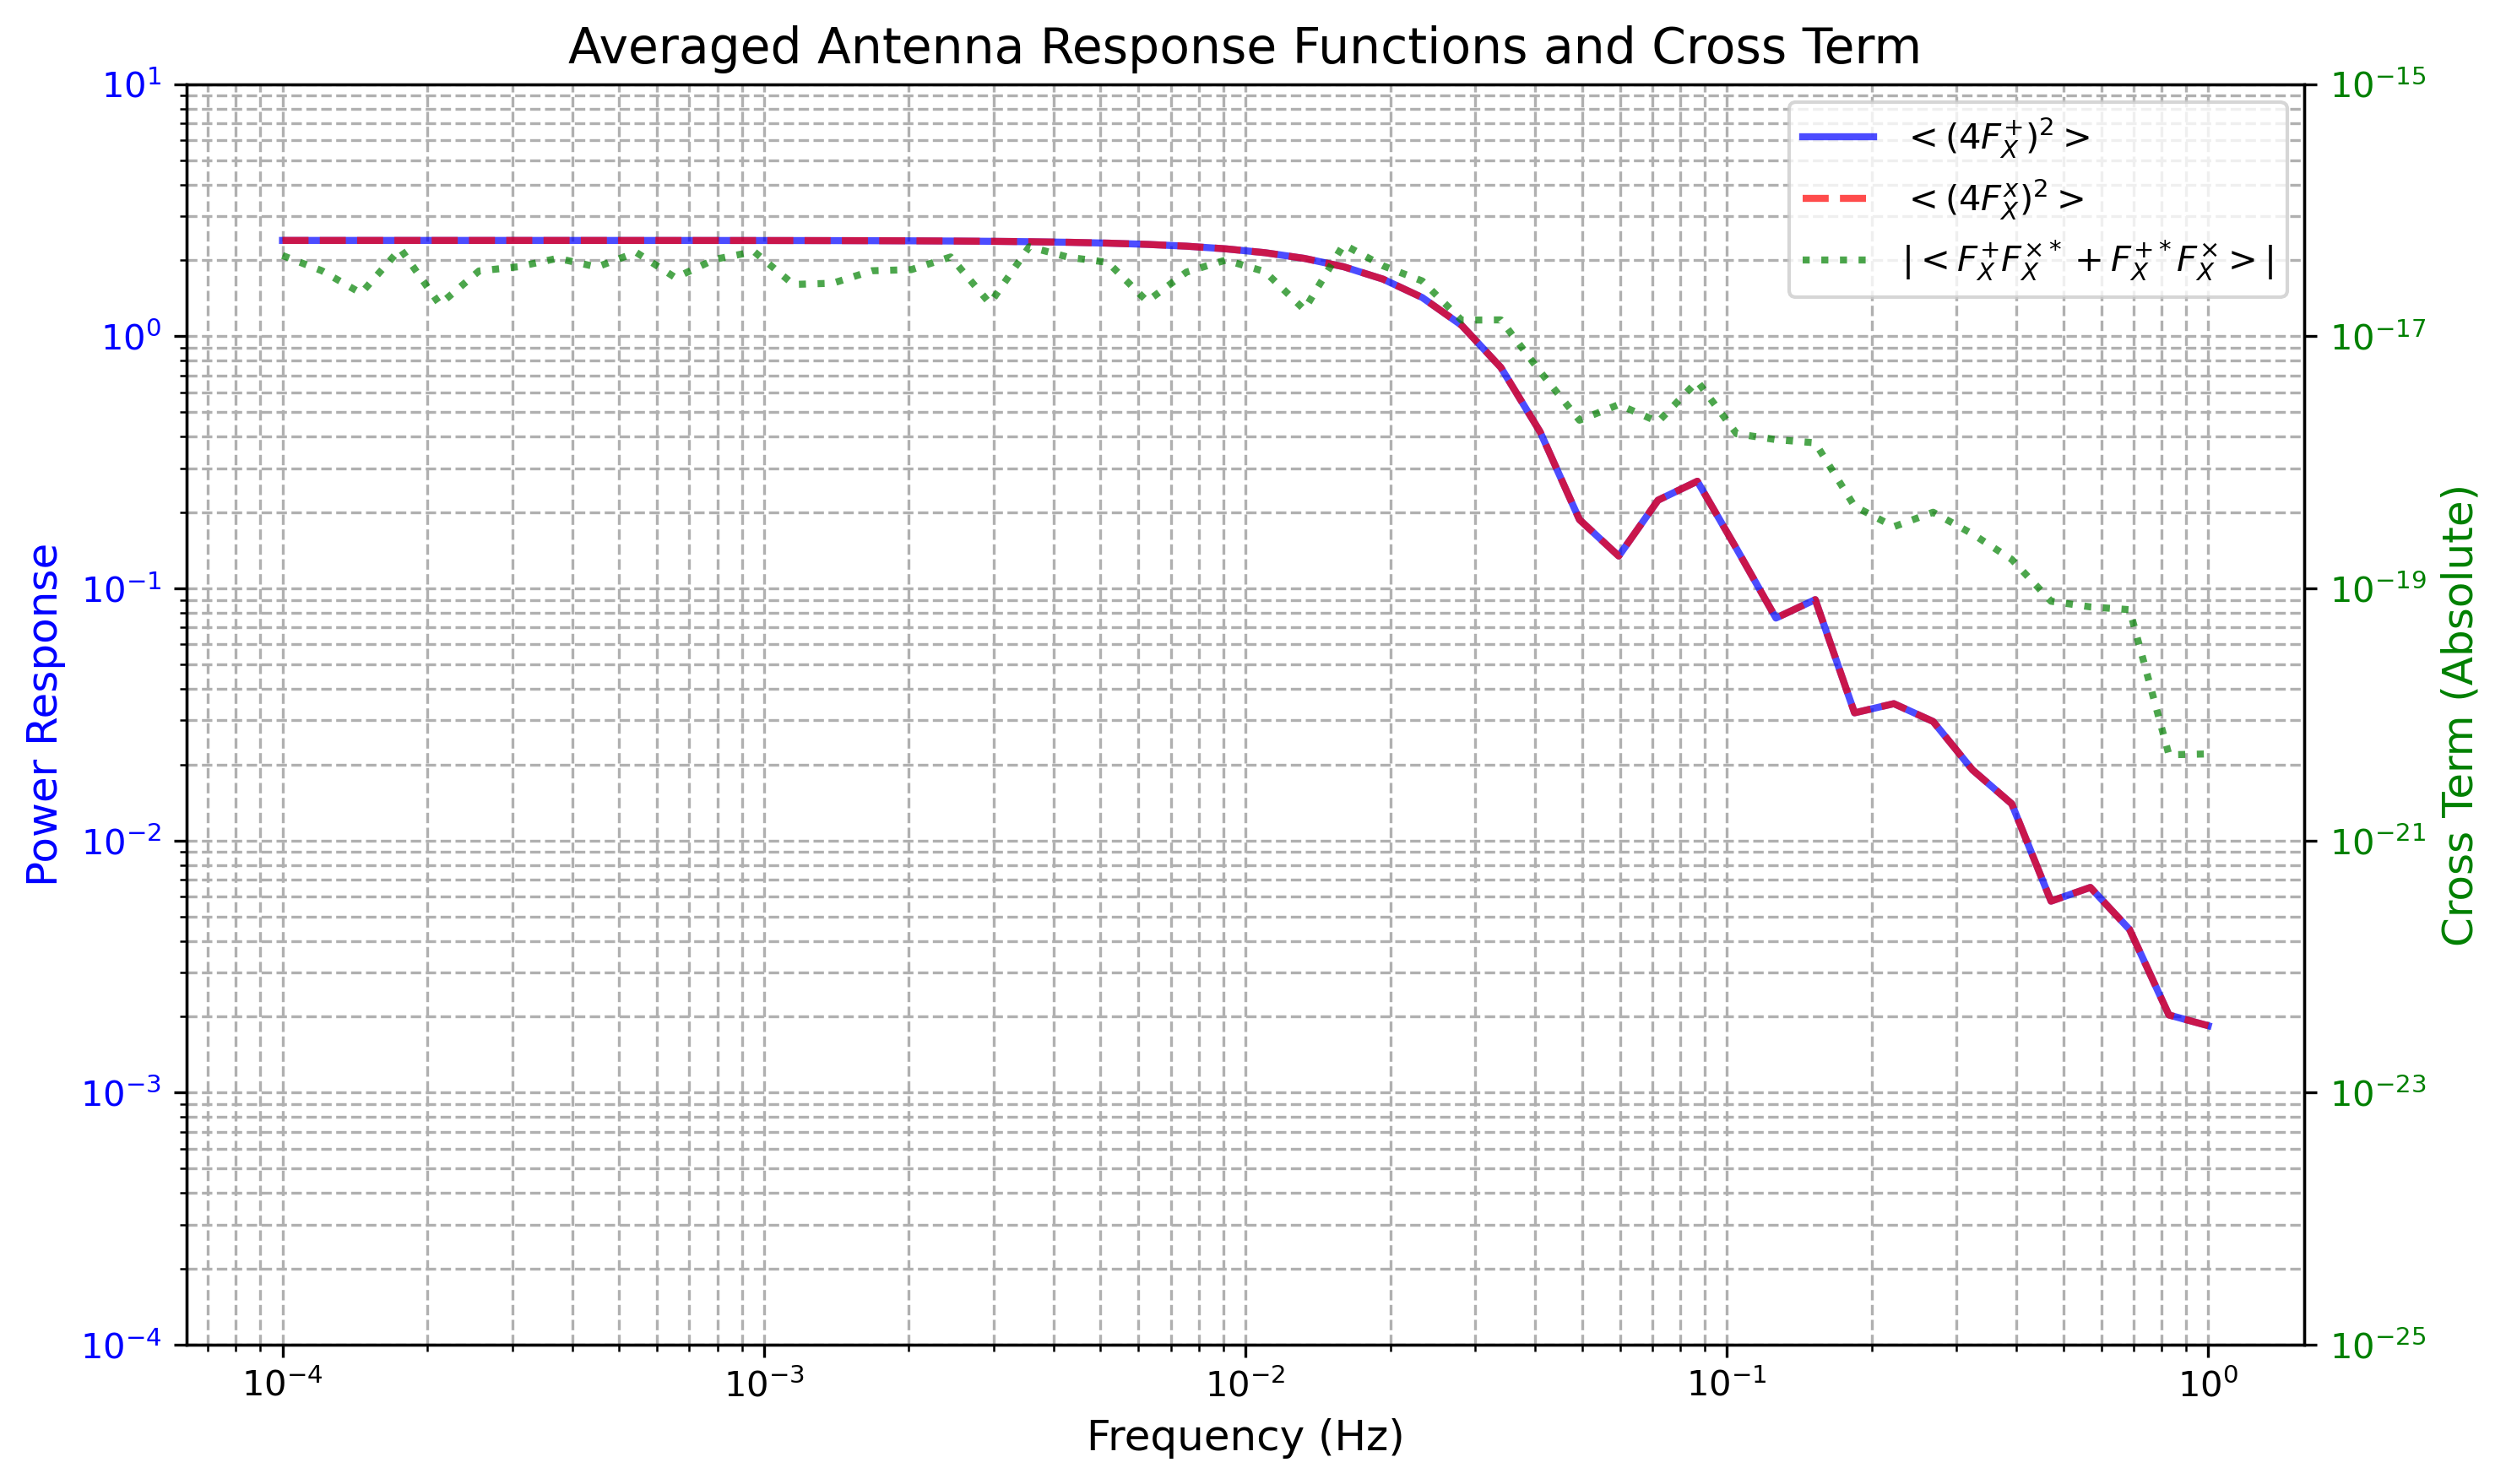
\includegraphics[width=0.7\linewidth]{mainfig}
		\caption{}
		\label{fig:semi}
	\end{figure}
	
	Next, we use this program to calculate $<F^{+}_{X} (F^{\times}_{X})^{*} + (F^{+}_{X})^{*} F^{\times}_{X}>$. The results, listed in Table \ref{tab:cross_term} showing near-zero values, indicate that $<F^{+}_{X} (F^{\times}_{X})^{*} + (F^{+}_{X})^{*} F^{\times}_{X}>$ is effectively 0 within the limits of numerical precision.
	
	
	\begin{table}[H]
		\centering
		\caption{The Cross-correlation Term}
		\label{tab:cross_term}
		\begin{tabular}{|c|c|}
			\hline
			Frequency (Hz) & $\langle\left| F^{+}_X (F^{\times}_X)^* + (F^{+}_X)^* F^{\times}_X \right|\rangle$ \\
			\hline
			$10^{-4}$ & $2.0795233272504503 \times 10^{-15}$ \\
			\hline
			$10^{-2}$ & $2.1172286586545604 \times 10^{-15}$ \\
			\hline
			1.0 & $1.9465964365455394 \times 10^{-18}$ \\
			\hline
		\end{tabular}
	\end{table}
	\label{tabcross}
	\title{}
	
	Substituting the above results into the equation \ref{X2.0}, we get the average response TDI X2.0 to GW:
	\begin{align}
		<\left|X^{GW}_{2.0}\right|^2> &= 64 (\omega L)^2 \sin^2 \omega L \sin^2 2 \omega L <(F^{+}_{X})^2> [A^2_{+} + A^2_{\times}] \\
		<R_{L,X_{2.0}} (f)> &= 64 (\omega L)^2 \sin^2 \omega L \sin^2 2 \omega L <(F^{+}_{X})^2>
	\end{align}
	
	\section{Approximation of $<(F^{+}_{X})^2>$}
	Now we need to compute the approximation of $<(F^{+}_{X})^2>$ at low frequencies $(\omega L << 1)$.
	
	For $X_{1.5}$TDI in the long wavelength limit(LISA-based frame) we obtain 
	\begin{equation}
		\tilde{X}_{1.5} \approx (4 \omega L) \sin \omega L \frac{\sqrt{3}}{2} (F_{+} \tilde{h}_{+} + F_{\times} \tilde{h}_{\times} )
	\end{equation} 
	where \begin{align}
		F_{+} &= -\frac{1}{2}(1 + \cos^2 \theta) \cos 2 \phi ~cos 2 \psi - \cos\theta ~\sin 2 \phi ~\sin 2 \psi \\
		F_{\times} &= \frac{1}{2}(1 + \cos^2 \theta) \cos 2\phi ~cos 2 \psi - \cos\theta ~\sin 2 \phi ~\cos 2 \psi
	\end{align}
	The value of $<(F_{+})^2>$ and $<(F_{\times})^2>$ is calculated to be 0.2. Using the definition:
	\begin{equation}
		SNR^2 = 4\text{Re}\left(\int_{0}^{f_{\text{max}}} df \frac{\tilde{X}\tilde{X}^*}{S_n(f)}\right)
	\end{equation}
	then:
	\begin{align}
		<SNR^2> &= <(F^{+}_{X})^2>\frac{3}{4}~ 4\text{Re} \left(\int_{0}^{f_{\text{max}}} df~(4\omega L)^2 \sin^2(\omega L) \frac{\tilde{h}^2_{+} + \tilde{h}^2_{\times}}{S_{n,X_{1.5}}(f)}\right) \\
		&= 4\text{Re} \left(\int_{0}^{f_{\text{max}}} df  (4\omega L)^2 \sin^2(\omega L) \frac{3}{20}\frac{\tilde{h}^2_{+} + \tilde{h}^2_{\times}}{S_{n,X_{1.5}}(f)}\right)
	\end{align}
	
	Using the definition:
	\begin{align}
		<SNR^2> &= 4\text{Re} \left( \int_{0}^{f_{\text{max}}} df \frac{\tilde{h}^2_{+} + \tilde{h}^2_{\times}}{S_n(f)/<\left|R_L\right|^2>} \right)
	\end{align}
	then:
	\begin{align}
		<\left| R^{LW}_{L,X_{1.5}} \right|^2> = \frac{3}{20} (4\omega L)^2 \sin^2(\omega L)
 	\end{align}
 	adding additional factor:
 	\begin{equation}
 		<\left| R_{L,X_{1.5}} \right|^2> = \frac{3}{20} (4\omega L)^2 \sin^2(\omega L) \frac{1}{1 + 0.6(\omega L)^2}
 	\end{equation}
 	That is to say:
 	\begin{equation}
 		<(4F^{+}_{X})^2> \approx 16 ~ \frac{3}{20} \frac{1}{1 + 0.6(\omega L)^2}
 	\end{equation}
 	Plotting to verify the accuracy of the approximation:
 	\begin{figure}[H]
 		\centering
 		\includegraphics[width=0.7\linewidth]{Numerical&approximation}
 		\caption{}
 		\label{fig:numericalapproximation}
 	\end{figure}
 	
 	\section{Finally compute the average response}
 	Using equation \ref{2.0}:
 	\begin{equation}
 		<\left| R_{L,X_{2.0}} \right|^2> = 64 (\omega L)^2 \sin^2 \omega L \sin^2 2 \omega L ~ \frac{3}{20} \frac{1}{1 + 0.6(\omega L)^2}
 	\end{equation}
 	The Average GW Response for TDI-X2.0 can be plotted:
 	\begin{figure}[H]
 		\centering
 		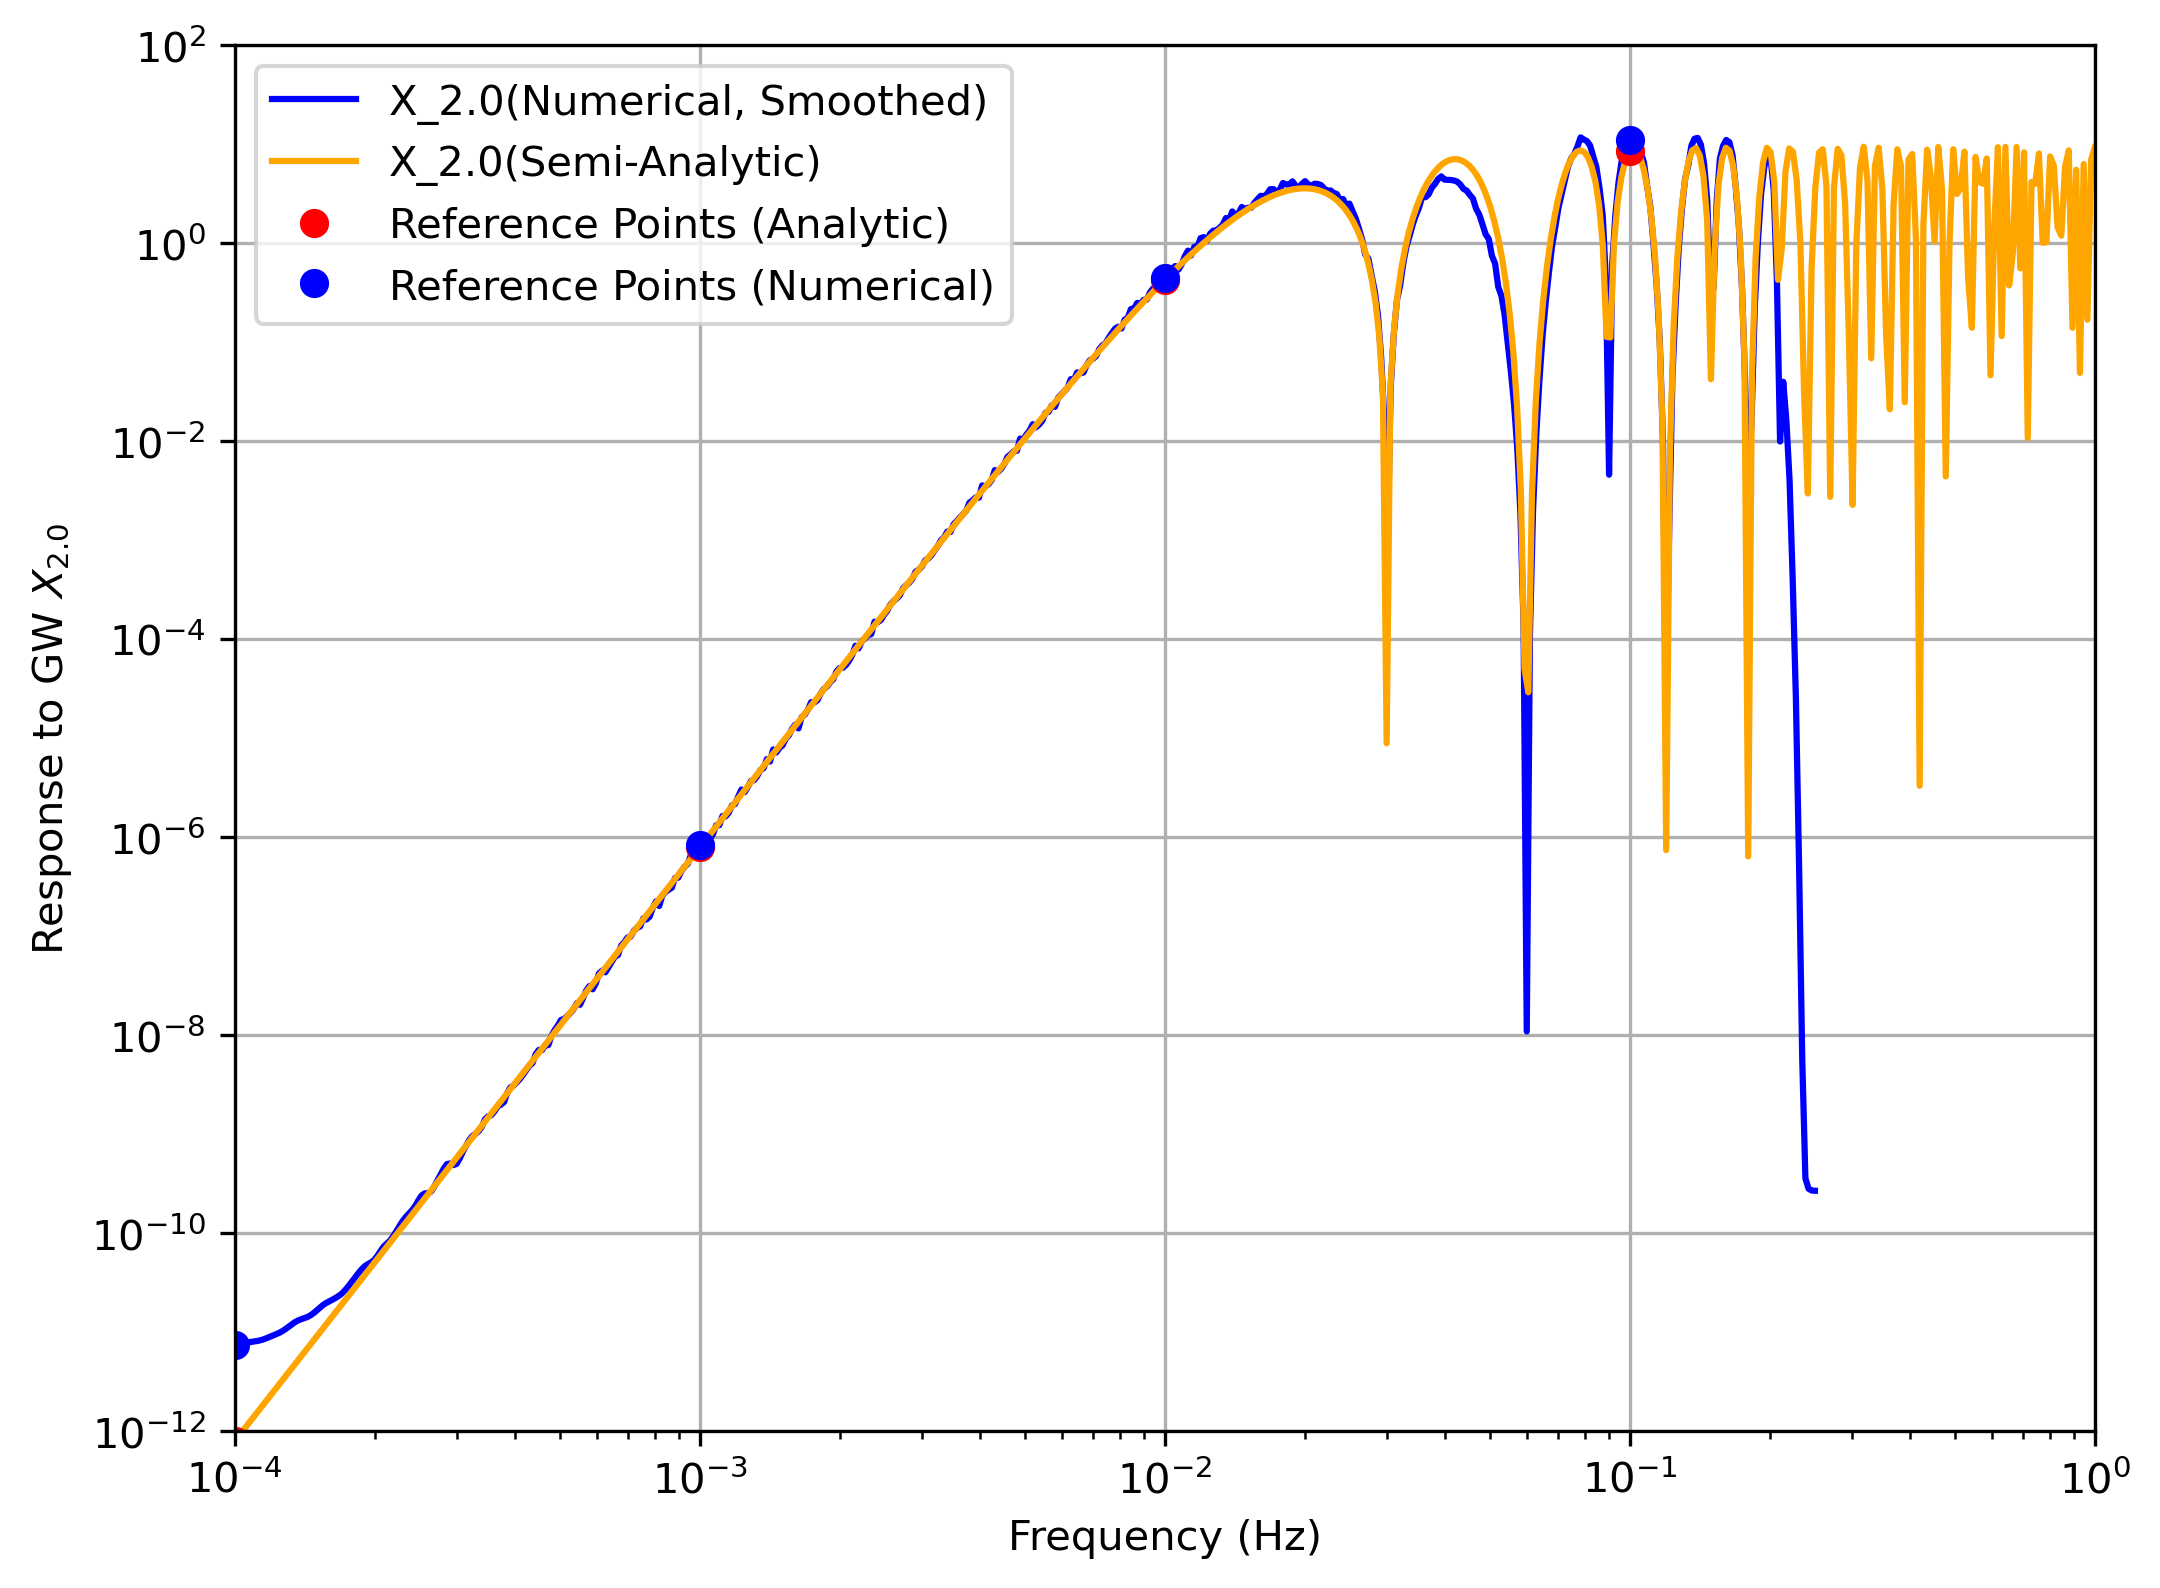
\includegraphics[width=0.7\linewidth]{numerical_semi_response}
 		\caption{The Average GW Response for TDI-X2.0}
 		\label{fig:numericalsemiresponse}
 	\end{figure}
 	
 	\begin{table}[H]
 		\centering
 		\caption{The numerical values of the response of TDI $X_{2.0}$ to GW for some fixed frequencies}
	\begin{tabular}{|c|c|c|}
		\hline
	Frequency (Hz) & Semi-Analytic & $R_{\text{LISACode},X_{2.0}}$ \\
	\hline
	0.00010 & 7.945098e-13 & 7.372150e-12 \\
	\hline
	0.00100 & 7.896301e-07 & 8.349357e-07 \\
	\hline
	0.01000 & 4.251647e-01 & 4.427565e-01 \\
	\hline
	0.10000 & 8.519737e+00 & 1.104438e+01 \\
	\hline
	\end{tabular}
   \end{table}
   
   \section{Sensitivity}
   Using the definition:
   \begin{align}
   	S_{h,X} &= \frac{S_{OMS} + (3 + \cos (2\omega L)) S_{acc}}{(\omega L)^2 <(F^+_x)^2>}\\
   	\sqrt{S_{OMS}}(f) &= 15\left[\frac{\text{pm}}{\sqrt{\text{Hz}}}\right] \sqrt{1 + \left(\frac{2\times10^{-3}}{f}\right)^4} \\
   	\sqrt{S_{acc}}(f) &= 3\left[\frac{\text{fm}.s^{-2}}{\sqrt{\text{Hz}}}\right] \sqrt{1 + \left(\frac{0.4\times10^{-3}}{f}\right)^2} \sqrt{1+\left(\frac{f}{8\times10^{-3}}\right)^4}
    \end{align}
    
    The strain sensitivity to only X, $\sqrt{S_{h,X}}$ can be plotted:
    \begin{figure}[H]
    	\centering
    	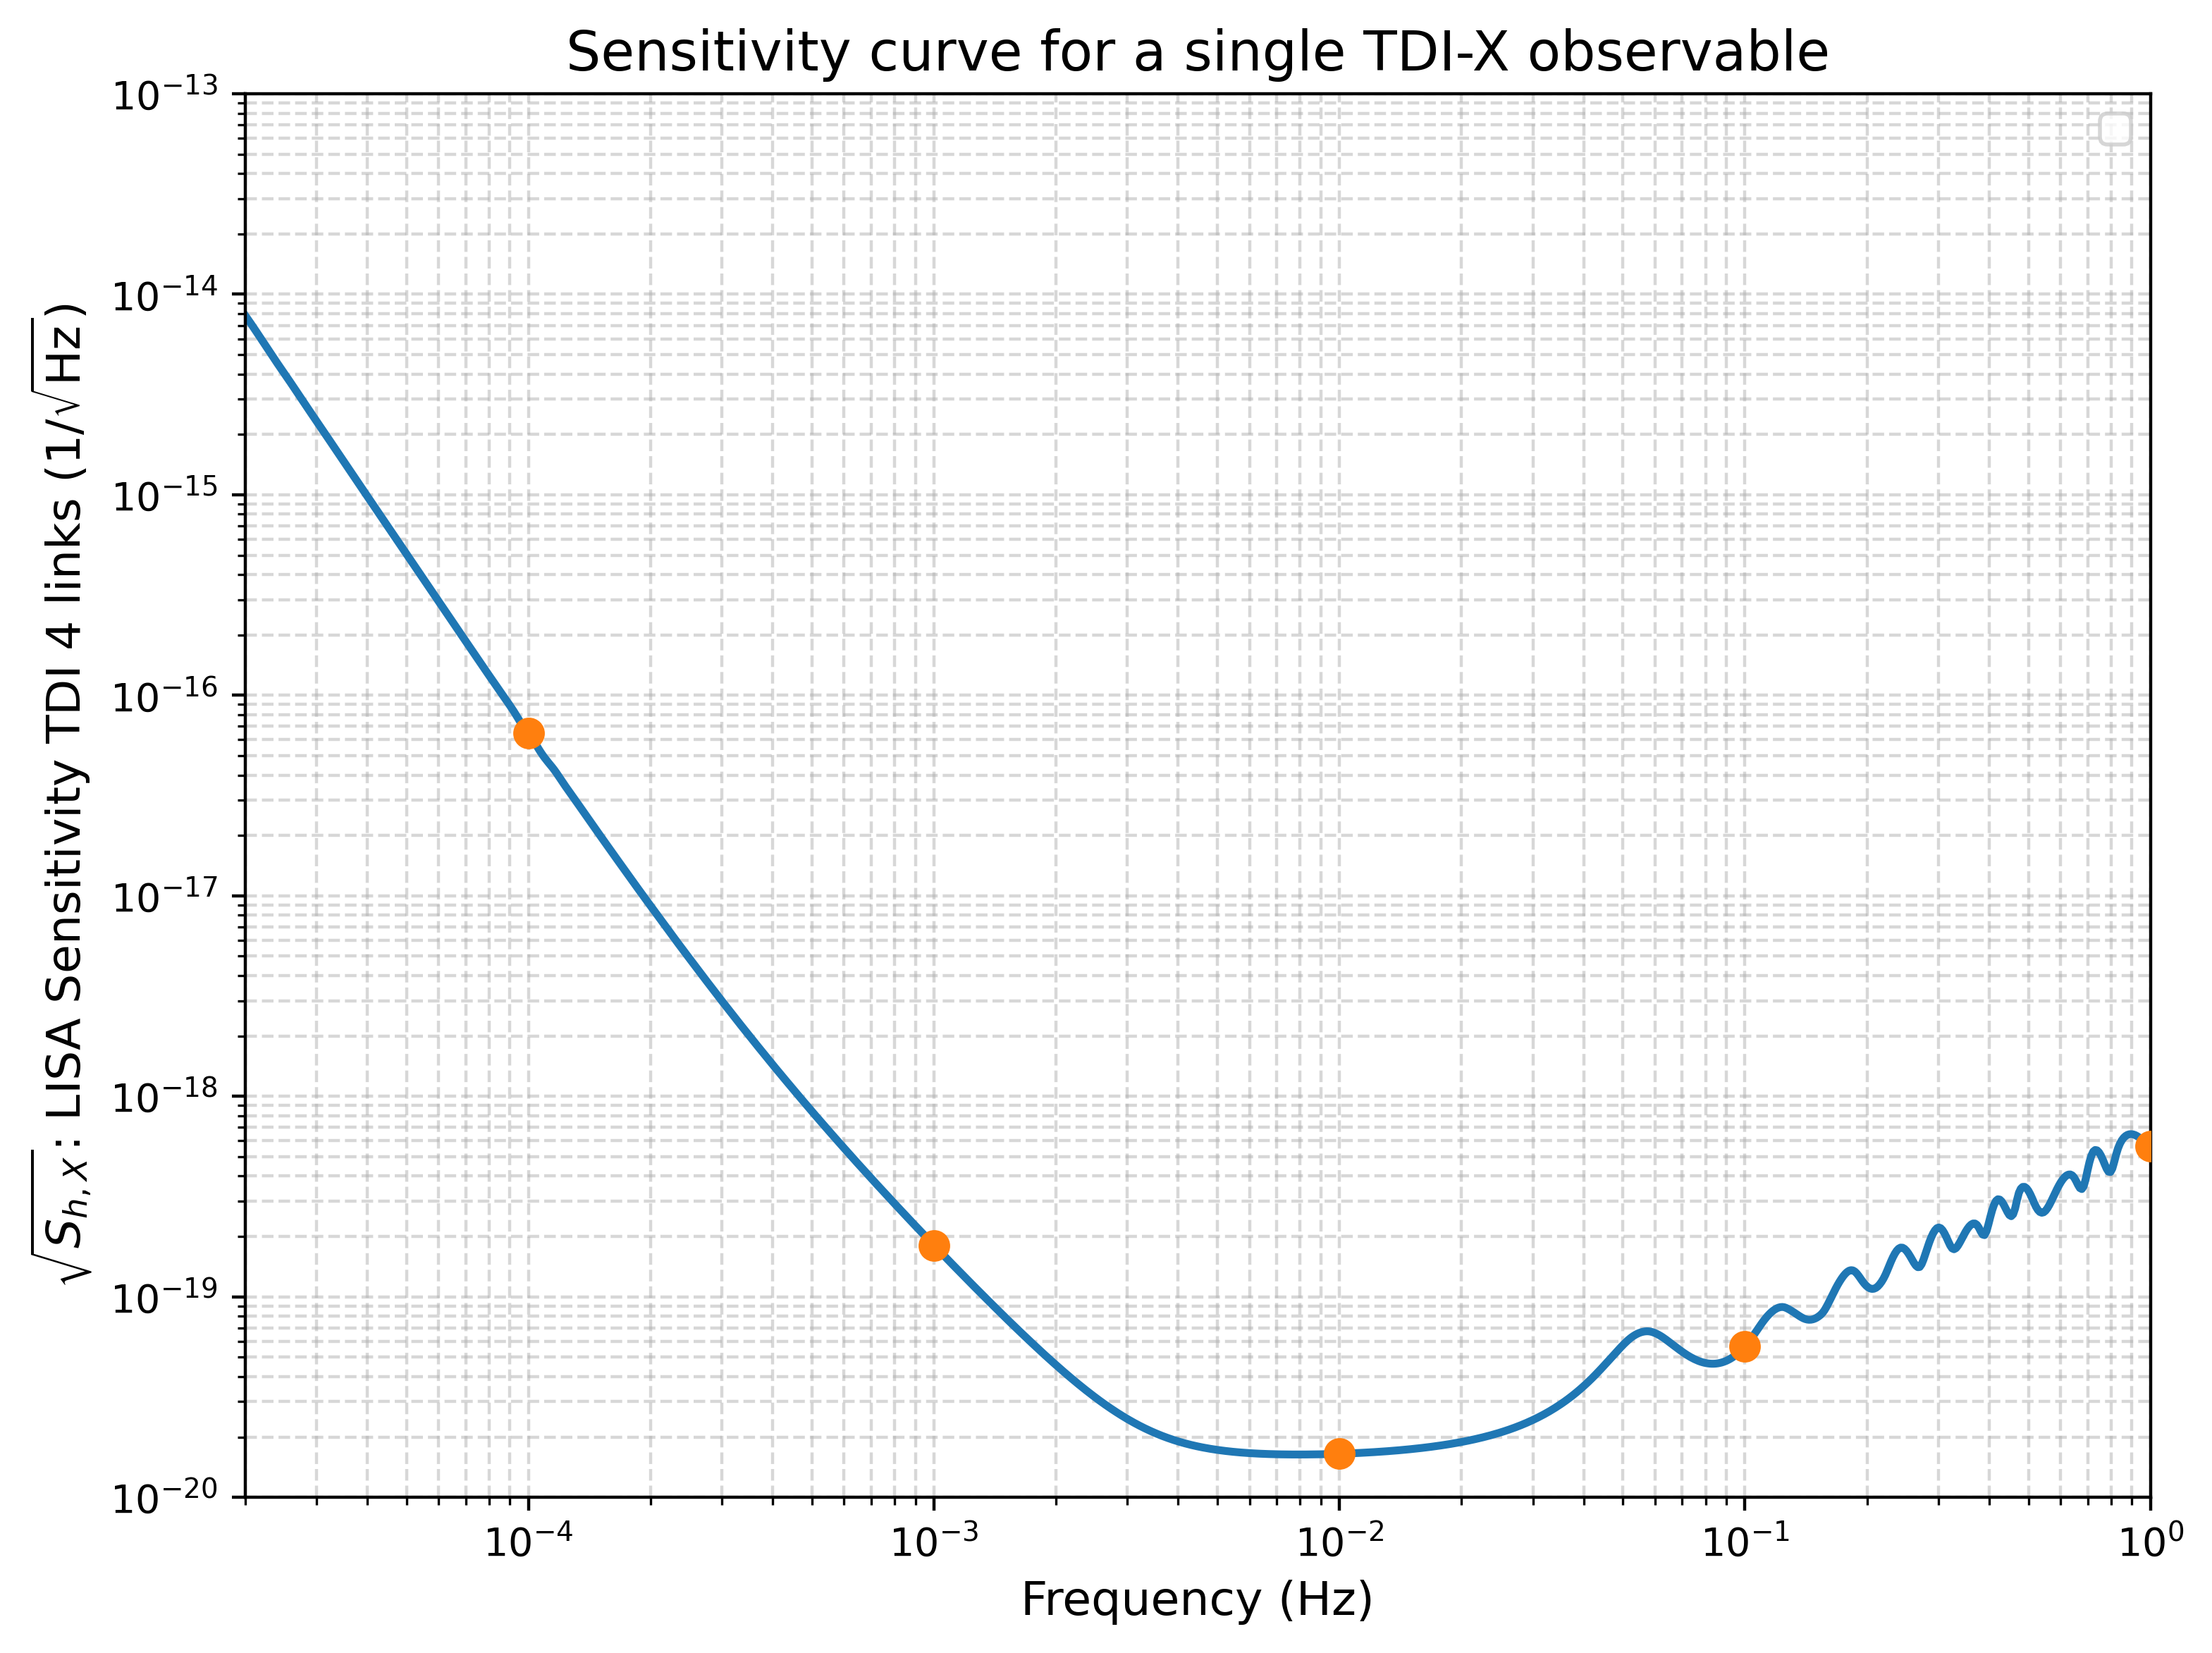
\includegraphics[width=0.7\linewidth]{sensitivity}
    	\caption{~}
    	\label{fig:sensitivity}
    \end{figure}
       
   \begin{table}[H]
   	\centering
   	\caption{The numerical values of the strain sensitivity curve for some fixed frequencies}
   	\begin{tabular}{|c|c|c|}
   		\hline
   		f (Hz) & $S_{h,X}$ & $S_{h}$ \\
   		\hline
   		0.00010 & 4.226903e-33 & 2.113451e-33 \\
   		\hline
   		0.00100 & 3.265832e-38 & 1.632916e-38 \\
   		\hline
   		0.01000 & 2.719033e-40 & 1.359516e-40 \\
   		\hline
   		0.10000 & 3.218440e-39 & 1.609220e-39 \\
   		\hline
   		1.00000 & 3.176069e-37 & 1.588034e-37 \\
   		\hline
   	\end{tabular}
   \end{table}
   
   
   
\end{document}

